\subsection{Direct Sparse Methods}
\subsubsection{Theory overview}

%%%%%%%%%%%%%%%%%%%%%%%%%%%%%%%%%%%%%%%%%%%%%%%%%%%%%%%%%%
\begin{frame}[t]{Direct Sparse Methods}
    \small
    \justifying
    
    Direct sparse methods combine the main advantages of direct and iterative methods
    
    \begin{itemize}
    	\item numerical accuracy of the methods is comparable with the standard Gaussian Elimination process
    	
    	\item complexity is bounded by $O(n^{2})$ due to efficient treatment of sparsity
    \end{itemize}

	\vspace{5mm}
	A solution of a system of equations is computed:
	\begin{itemize}
		\item by means of forward and backward substitutions
		 
		\item using $LU$ decomposition of the corresponding matrix.
	\end{itemize}
\end{frame}


\begin{frame}[t]{Direct Sparse Methods: Speech}
	\small
	\justifying
	\begin{itemize}
		\item The multifrontal method is probably the most representative example of direct sparse solvers
		 introduced by Duff and Reid
		 
		 \item The method is an improved version of the frontal method 
		 
		 \item which can compute independent fronts in parallel. 
		 
		 \item A front, also called a frontal matrix, can be considered as a small dense matrix 
		 
		 \item resulting from a column elimination of the original system. 
		 
		 \item There also exist left- and right-looking vatiants of the multifrontal method
		 
	\end{itemize}

	\vspace{5mm}
	Let's consider the multifrontal methods as an example\\
	\vspace{2.5mm}
	To keep the overview rather simple, we assume that matrix $A$ is \textbf{symmetric positive definite} and \textbf{sparse}
	
	
	
\end{frame}


\begin{frame}[t]{Multifrontal Method: I}
	\small
	\justifying
		\begin{equation} \label{eq:chol-1}
		A = LDL^T \qquad \text{with}\quad (D)_{ii} > 0
		\end{equation}
		
		Given a rule and a sparsity pattern, one can build an elimination tree
		\begin{equation} \label{eq:elimination-tree-1}
			p = min(i > j | l_{ij} \neq 0)
		\end{equation}
		
	
	\vspace{-5mm}
		
	\begin{columns}
		\begin{column}{0.5\textwidth}
			\begin{figure}[!htpb]
				\centering
				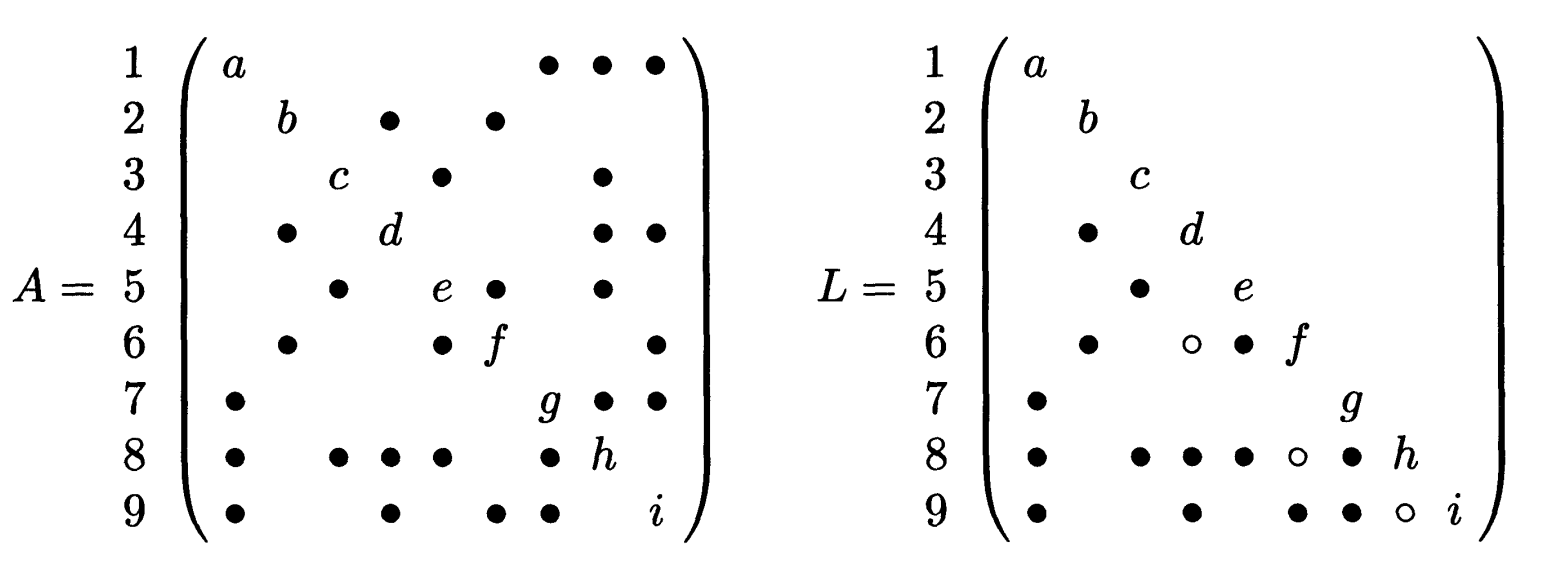
\includegraphics[width=1.2\textwidth]{figures/chapter-2/sparsity-pattern-example-mm.png}
				\caption{A sparse matrix and its Cholesky factor, \cite{mult-frontal-original:2}}
				\label{fig:sparsity-pattern-example-mm}
			\end{figure}
		\end{column}
			
		\begin{column}{0.5\textwidth}
			
			\begin{figure}[!htpb]
				\centering
				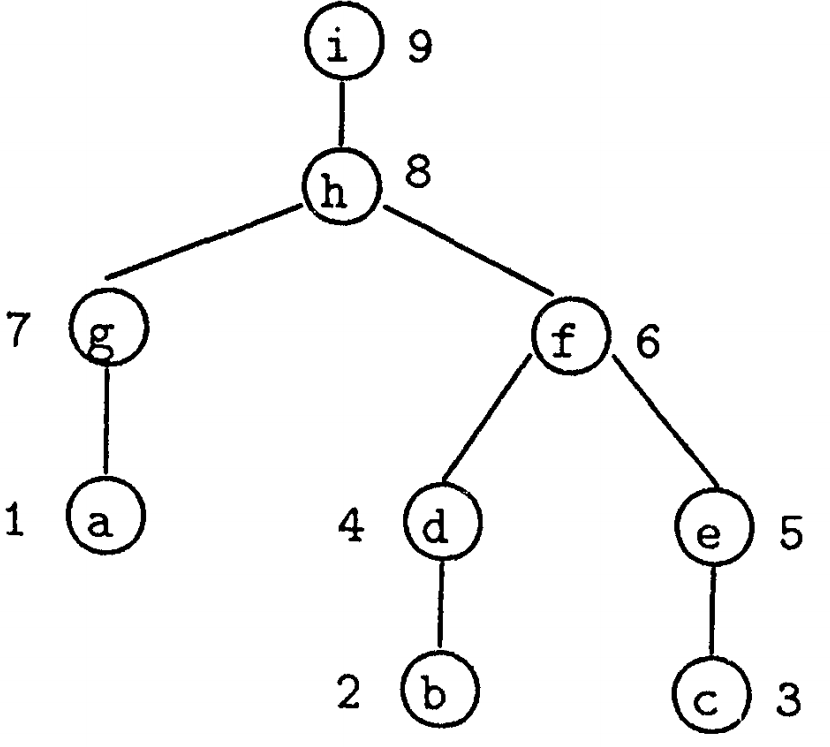
\includegraphics[width=0.65\textwidth]{figures/chapter-2/elimination-tree-mm.png}
				\caption{An elimination tree, \cite{mult-frontal-original:2}}
				\label{fig:elimination-tree-mm}
			\end{figure}
		\end{column}

	\end{columns}
	
	
\end{frame}


\begin{frame}[t]{Multifrontal Method: II}
	\small
	\justifying
	The fundamental idea of the multifrontal method spins around frontal $F$ and update matrices $\hat{U}$
	\begin{equation} \label{eq:mm-1}
		F_{j} = Fr_{j} + \hat{U_{j}} = \begin{bmatrix}a_{j,j} & a_{j,i_1} & a_{j,i_2} & \dots & a_{j,i_r} \\
		a_{i_1,j} \\
		a_{i_2,j} \\
		\vdots & & & 0\\
		a_{i_r,j} \\
		\end{bmatrix} + \hat{U_{j}}
	\end{equation}
	
	where $i_{0}$, $i_{1}$, $i_{2}$, \dots , $i_{r}$ are row subscripts of non-zeros in $L_{*j}$ where $i_{0} = j$; $r$ is the number of off-diagonal non-zero elements.\\


	\begin{equation} \label{eq:mm-2}
		\hat{U_{j}} = - \sum_{k \in T[j] -{j}}  \begin{bmatrix}
		l_{j,k} \\
		l_{i_1,k} \\
		\vdots \\
		l_{i_r,k} \\
		\end{bmatrix} \begin{bmatrix}
		l_{j,k} & l_{i_1,k} & \dots & l_{i_r,k}
		\end{bmatrix} 
	\end{equation}
	
	where $\hat{U_{j}}$ can be treated as the second term of the Schur complement
	
\end{frame}


\begin{frame}[t]{Multifrontal Method: III}
	\small
	\justifying
	Let's consider factorization of a 2-by-2 block matrix $A$
	\begin{equation} \label{eq:mm-3}
		A = \begin{bmatrix}
		B & V^{T} \\
		V & C
		\end{bmatrix} 
		= 
		\begin{bmatrix}
		L_{B} & 0 \\
		VL^{-T}_{B} & I
		\end{bmatrix}
		\begin{bmatrix}
		I & 0 \\
		0 & Sr
		\end{bmatrix} 
		\begin{bmatrix}
		L^{T}_{B} & L^{-1}_{B}V^{T} \\
		0 & I
		\end{bmatrix} 
	\end{equation}
	
	Assuming that block $B$ has already been factorized: $B = L_{B}L^{T}_{B}$\\
	
	\vspace{5mm}
	The Schur complement can be viewed as:
	\begin{equation} \label{eq:mm-3}
	Sr =  C - VB^{-1}V^{T}
	\end{equation}
	
	\begin{columns}
		\begin{column}{0.5\textwidth}
			\textit{Dense Linear Algebra:} $-VB^{-1}V^{T}$\\
			\begin{equation} \label{eq:mm-5}
				-\sum_{k=1}^{j-1}  \begin{bmatrix}
				l_{j,k} \\
				\vdots \\
				l_{n,k} \\
				\end{bmatrix} \begin{bmatrix}
				l_{j,k} & \dots & l_{n,k}
				\end{bmatrix} 
			\end{equation}
		\end{column}
	
		\begin{column}{0.5\textwidth}
			\textit{Multifrontal method:} $\hat{U_{j}}$\\
			\begin{equation} \label{eq:mm-2}
				-\sum_{k \in T[j] -{j}}  \begin{bmatrix}
				l_{i_0,k} \\
				\vdots \\
				l_{i_r,k} \\
				\end{bmatrix} \begin{bmatrix}
				l_{i_0,k} & \dots & l_{i_r,k}
				\end{bmatrix} 
			\end{equation}
		\end{column}
	\end{columns}
	
\end{frame}


\begin{frame}[t]{Multifrontal Method: IV}
	\small
	\justifying
	
	After column $j$ factorization:
	\begin{equation} \label{eq:mm-6}
		\hat{F_{j}} = \begin{bmatrix}
		l_{j,j} & \dots & 0 \\
		\vdots & I \\
		l_{i_{r},j} \\
		\end{bmatrix} 
		\begin{bmatrix}
		1 & \dots & 0 \\
		\vdots & U_{j} \\
		0 \\
		\end{bmatrix} 
		\begin{bmatrix}
		l_{j,j} & \dots & l_{i_{r},j} \\
		\vdots & I \\
		0 \\
		\end{bmatrix} 
	\end{equation}
	where sub-matrix $U_{j}$ represents the full update from all descendants of node $j$ and node $j$ itself
	
	
	\begin{columns}
		
	\begin{column}{0.25\textwidth}
		\begin{figure}[!htpb]
			\centering
			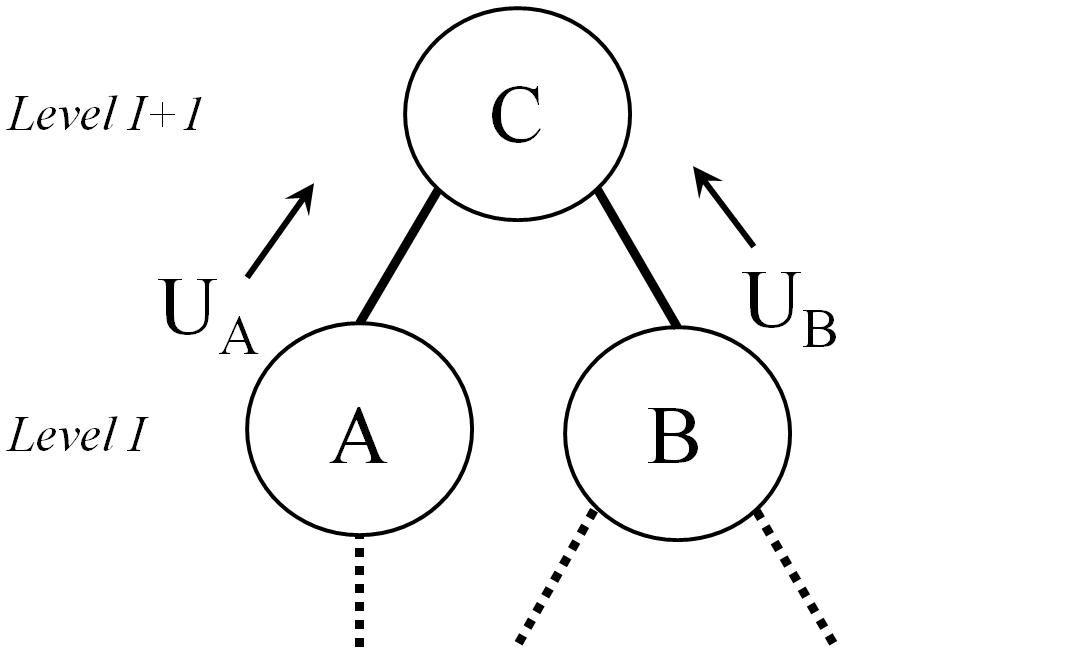
\includegraphics[width=1.35\textwidth]{figures/chapter-2/information-flow.png}
			\caption{Information flow}
			\label{fig:information-float}
		\end{figure}
	\end{column}

	\begin{column}{0.75\textwidth}
		\begin{equation} \label{eq:mm-9}
			F_{j} = \begin{bmatrix}a_{j,j} & a_{j,i_1} & a_{j,i_2} & \dots & a_{j,i_r} \\
			a_{i_1,j} \\
			a_{i_1,j} \\
			\vdots & & & 0\\
			a_{i_r,j} \\
			\end{bmatrix} \extendadd U_{c_1} \extendadd \dots \extendadd U_{c_s} 
		\end{equation}
	\end{column}

	\end{columns}
\end{frame}



\begin{frame}[t]{Supernodal Method}
	\small
	
	\begin{itemize}
		\item In practice, an improved version of the multifrontal method is used
		\item A super-node is formed by a set of contiguous columns 
		
		\item which have the same  off-diagonal sparsity structure
	\end{itemize}

	\begin{equation} \label{eq:mm-10}
		\mathcal{F}_{j} = \begin{bmatrix}a_{j,j} & a_{j,j+1} & \dots & a_{j,j+t}  & a_{j,i_1} & \dots & a_{j,i_r} \\
		a_{j+1,j} & a_{j+1,j+1} & \dots & a_{j+1,j+t}  & a_{j+1,i_1} & \dots & a_{j+1,i_r} \\
		\vdots & \vdots & \dots & \vdots \\
		a_{j+t,j}  & a_{j+t,j+1} & \dots & a_{j+t,j+t}  & a_{j+t,i_1} & \dots & a_{j+t,i_r} \\
		a_{i_1,j} & a_{i_1,j+1} & \dots & a_{i_1,j+t} \\
		\vdots & \vdots & \dots & \vdots  & & 0\\ 
		a_{i_r,j} & a_{i_r,j+1} & \dots & a_{i_r,j+t} \\
		\end{bmatrix} \extendadd U_{c_1} \dots \extendadd U_{c_s} 
	\end{equation}

\end{frame}